\chapter{Атом}\label{ch:atom}

\epigraph{\emph{Величайшим достижением человеческого гения является то, что человек может понять вещи, которые он уже не в силах вообразить.}}
{Лев Ландау}


Идея об атоме прошла извилистый и местами весьма драматический путь, прежде чем приобрела тот вид, в котором ее изучают сегодня в школах и университетах.
Довольно простая и естественная мысль о существовании небольшого числа одинаковых элементов в итоге привела к совершенно удивительным открытиям.
Все новые и новые факты об атоме, сформировавшие в начале XX века фундамент ядерной физики, поначалу скорее все больше запутывали ученых, нежели вносили ясность.
Оказалось, что знания о микромире попросту нельзя получать и интерпретировать классическим методом, используя интуицию и сравнение с какими-либо привычными объектами вроде стальных шариков или планет Солнечной системы.
Атом оказался чем-то совершенно иным.
Как писал Нильс Бор, ``если ты не шокирован квантовой физикой — ты ее еще не понял''.

Открытие и научное описание процесса деления атомного ядра стало кульминацией всей истории проникновения в тайны атома. 
Именно возможность искусственного расщепления ядер позволило освободить огромную энергию, скрытую внутри вещества.
Может вызывать некоторый дискомфорт мысль о том, что это по-настоящему великое открытие впервые было применено именно в военных целях, в одно мгновение унеся жизни сотен тысяч людей.
Но таков путь истории, и его не изменить.

Здесь мы просуммируем основные факты об атоме и процессе его деления, необходимые для понимания математики, позволяющей его точно описать.
Нам не потребуются ни глубокие знания современной ядерной физики, ни сложный математический аппарат квантовой механики.
Для наших целей будет вполне достаточно общих знаний о строении атома и ядерных реакциях.
Без них было бы крайне тяжело понять, почему те или иные задачи ставились перед физиками и математиками Манхэттенского проекта.
Многие из излагаемых ниже фактов были хорошо им известны и с того времени практически не изменились.  
Этих знаний оказалось вполне достаточно для реализации основной цели проекта - создания ядерного оружия.
Более глубокие факты об атоме вроде строения нкулонов были открыты позднее и приводятся здесь лишь в самых общих чертах и только для полноты общей картины.


\section*{Строение}

Итак, что же такое атом? 
К настоящему времени известно следующее.
Атом - микроскопическая частица вещества, состоящая из тяжелого ядра, окруженного легкими по сравнению с ним электронами.
Ядро состоит из нуклонов - протонов и нейтронов, находящихся практически в непосредственной близости друг о друга.

Протоны и нейтроны очень похожи друг на друга.
Они имеют практически идентичное внутреннее строение и отличаются по массе лишь на одну десятую процента.
Главное отличие между ними - электрический заряд, положительный у протона, и полностью отсутствующий у нейтрона.

\begin{figure}[t!]
   \centering
   \includegraphics[scale=0.5]{images/atom_1}
   \caption{Строение атома гелия: два протона и нейтрона в ядре и два электрона, ``размазанные'' около ядра в облаке формы шарового слоя. Наиболее вероятное местонахождение электронов - пунктирная сфера, но точно локализовать электрон в пространстве невозможно.}
   \label{fig:atom_1}
\end{figure}

На рис. \ref{fig:atom_1} схематически изображен атом гелия.
Он имеет два протона и нейтрона в ядре и два электрона на некотором расстоянии от центра.
В реальности электроны располагаются на очень большом отдалении от ядра - в десятки-сотни тысяч раз большем, чем его диаметр.

Заряд электрона - отрицательный и равный по абсолютной величине заряду протона.
Число электронов при этом равно числу протонов в ядре, что гарантирует электронейтральность атома в целом.
Последнее отнюдь не означает, что атом в процессе жизни не может потерять или приобрести электрон.
Это вполне возможно, и атом при этом приобретает положительный или отрицательный заряд, становясь \textit{ионом}.
Нас будут интересовать только электронейтральные атомы.

Таким образом, несмотря на неоправдавшуюся мечту об идеальности и неделимости, оказалось, что атом сам по себе устроен довольно просто и элегантно.
Как выяснилось позднее, основные сложности кроются еще на уровень глубже.
Насколько просто строение атома в целом, настолько же сложным оказалось внутреннее устройство и поведение его отдельных частей: протонов, нейтронов и электронов.
Именно здесь и начинаются главные сложности, не до конца ясные даже сегодня.
Дело в том, что протоны и нейтроны в свою очередь состоят из еще более мелких субатомных частиц - кварков, которые до сих пор порождают больше вопросов, чем ответов.
По словам современного физика Мэтта Страсслера, ``устройство атома напоминает легкий и элегантный танец, тогда как устройство протона - сумасшедшую вечеринку''.

С электронами тоже оказалось не все так просто.
Положение электронов в пространстве относительно ядра невозможно точно определить, о чем подробнее рассказано ниже.
Интересно, что как электроны, так и кварки вполне могут оказаться действительно \textit{элементарными} частицами, то есть не имеющими размеров и далее неделимыми на более мелкие еще неизвестные науке частицы.
Пока это точно установить не удалось.

Число протонов в ядре называется \textit{атомным номером} химического элемента.
Оно однозначно определяет его тип и место в периодической таблице элементов: водород - один протон, гелий - два протона и так далее.
Число нейтронов в атоме элемента при этом может быть любым, но обычно не слишком отличается от числа протонов.
Суммарное количество протонов и нейтронов называют \textit{массовым числом} атома.
Например, запись $\ce{^{235}_{92}U}$ обозначает химический элемент уран с массовым числом 235, имеющий в своем ядре 92 протона и 143 нейтрона.

Для одного и того же элемента с разным числом нейтронов говорят о его \textit{изотопах}.
Примечательно, что изотопы одного и того же элемента отличаются только своей массой, но не химическими свойствами.
Таким образом, именно число протонов в ядре атома дает ему химическую индивидуальность.
Главное, помимо массы, различие изотопов одного элемента - их стабильность, о чем подробно рассказано ниже.

Обычно в природе широко распространен какой-то один изотоп каждого химического элемента.
Этот изотоп обнаруживается в подавляющем числе случаев и имеет долгое время жизни.
Остальные изотопы очень редки, либо синтезируются искусственно и имеют очень малое время жизни. 

Например, атом с одним протоном и без нейтронов в ядре представляет тот же самый химический элемент, что и атомы с одним протоном и одним, двумя или тремя нейтронами. 
Это первые изотопы водорода - протий \ce{^{1}_{1}H}, дейтерий \ce{^{2}_{1}H}, тритий \ce{^{3}_{1}H} и квадий \ce{^{4}_{1}H}.
Самый легкий и стабильный из них - протий - встречается в природе в $99.98\%$ случаев.
Квадий синтезирован искусственно и крайне нестабилен.


\section*{Электронное облако}

Главный и наиболее сложный для понимания факт об электронах в атоме состоит в том, что их точное местоположение указать невозможно.
Они как бы размазаны в пространстве около ядра, образуя \textit{электронное облако} - довольно причудливый трехмерный объект с областями большей и меньшей плотности.

На рис. \ref{fig:atom_1} схематически изображено облако двух электронов атома гелия.
Оно представляет собой сферически симметричную область в пространстве, наиболее плотную в окрестности сферы с центром в ядре атома.
На рисунке это наиболее темная область, выделенная для наглядности пунктиром.
Сами точечные электроны на рисунке - скорее схематическая абстракция, нежели реальные точечные объекты.
Их точное местоположение не определено ни в какой момент времени - они могут находиться практически где угодно, но вероятнее всего - в более темных областях около пунктирной линии.
Подобное поведение физических объектов не встречается нигде в привычных нам наблюдаемых явлениях в обычной жизни.
Оно уникально для микромира. 

Остановимся на этом удивительном факте подробнее.
Принципиально здесь то, что неопределенность положения электрона данном случае отражает не наше субъективное временное незнание, а объективный факт: положение электрона в пространстве невозможно точно определить никакими инструментами и расчетами.
Первое приходящее на ум объяснение этому странному явлению - мы пока просто не располагаем инструментами необходимой точности, и они когда-нибудь появятся в будущем.
Но это не так.
Невозможность точно локализовать электрон принципиальна и никак не зависит от наших технических возможностей.

Разница между субъективной и объективной неопределенностью хорошо видна на следующем примере.
Предположим, мы подбрасываем монетку и интересуемся, какой стороной она выпадет.
Если монетка честная, то примерно в половине случаев она будет выпадать орлом, и примерно в половине - решкой.
Подбрасывая монетку, мы действительно заранее не знаем результат и говорим лишь о вероятности выпадения, например, орла.
Но в этом случае мы все-таки могли бы точно предсказать результат, если бы заранее знали силу и скорость броска, а также точные турбулентные движения воздуха около монетки.
Иными словами, при желании мы могли бы полностью устранить неопределенность результата броска монетки, выписав и решив полную систему уравнений ее движения (неоправданно сложную для столь скромных целей, но тем не менее). 

С электроном все обстоит иначе.
Мы полностью лишены возможности обладания некой дополнительной скрытой информацией вроде движения воздуха вокруг монетки в приведенном примере, которая в итоге позволила бы точно определить его местонахождение.
Ученые потратили огромное количество усилий, пытаясь найти подобные \textit{скрытые переменные}, и у них ничего не вышло.
Пришлось признать (и тому есть другие подтверждения), что электрон существует сразу везде, просто где-то с большей вероятностью. 
Распределенное в пространстве состояние - это естественный способ существования электрона в этом мире.
Так он устроен, и ничего с этим не поделаешь. 

Смирившись с невозможностью определить точное положение электрона в пространстве, можно попытаться задаться вопросом о нахождении по крайней мере этой самой вероятности обнаружить его в определенном месте.
Это отнюдь не бесполезная работа.
Мы видели, что в каких-то областях шанс обнаружить электрон выше, а значит должна быть возможность как-то это количественно описать.
Это, конечно, будут не точные координаты электрона, но уже и не полная неопределенность.

Для описания такого рода частичных неопределенностей в математике используются специальные объекты - \textit{плотности распределения вероятностей}.
Это числовые функции, принимающие б'ольшие значения там, где вероятность должна быть выше (подробнее о плотностях см. главу ….).
Таким образом, в нашем случае можно сказать, что электрон (даже один единственный!) \textit{распределен} в пространстве так, что его скорее обнаружить там, где значение этой функции больше.
С визуальной точки зрения электронное облако электрона оказывается плотнее там, где больше его функция плотности (см. рис. \ref{fig:atom_1}).
Эту функцию принято еще называть \textit{орбиталью} электрона в атоме.

Итак, мы связали нашу новую интуицию о положении электрона в пространстве с конкретным математическим объектом - орбиталью. 
Откуда же можно ее получить?
Оказывается, это вполне возможно сделать точно, решив специальное уравнение - уравнение Шреддингера.
Это довольно сложный математический объект, подробнее о котором рассказано в необязательной дополнительной главе ....

\begin{figure}[t!]
   \centering
   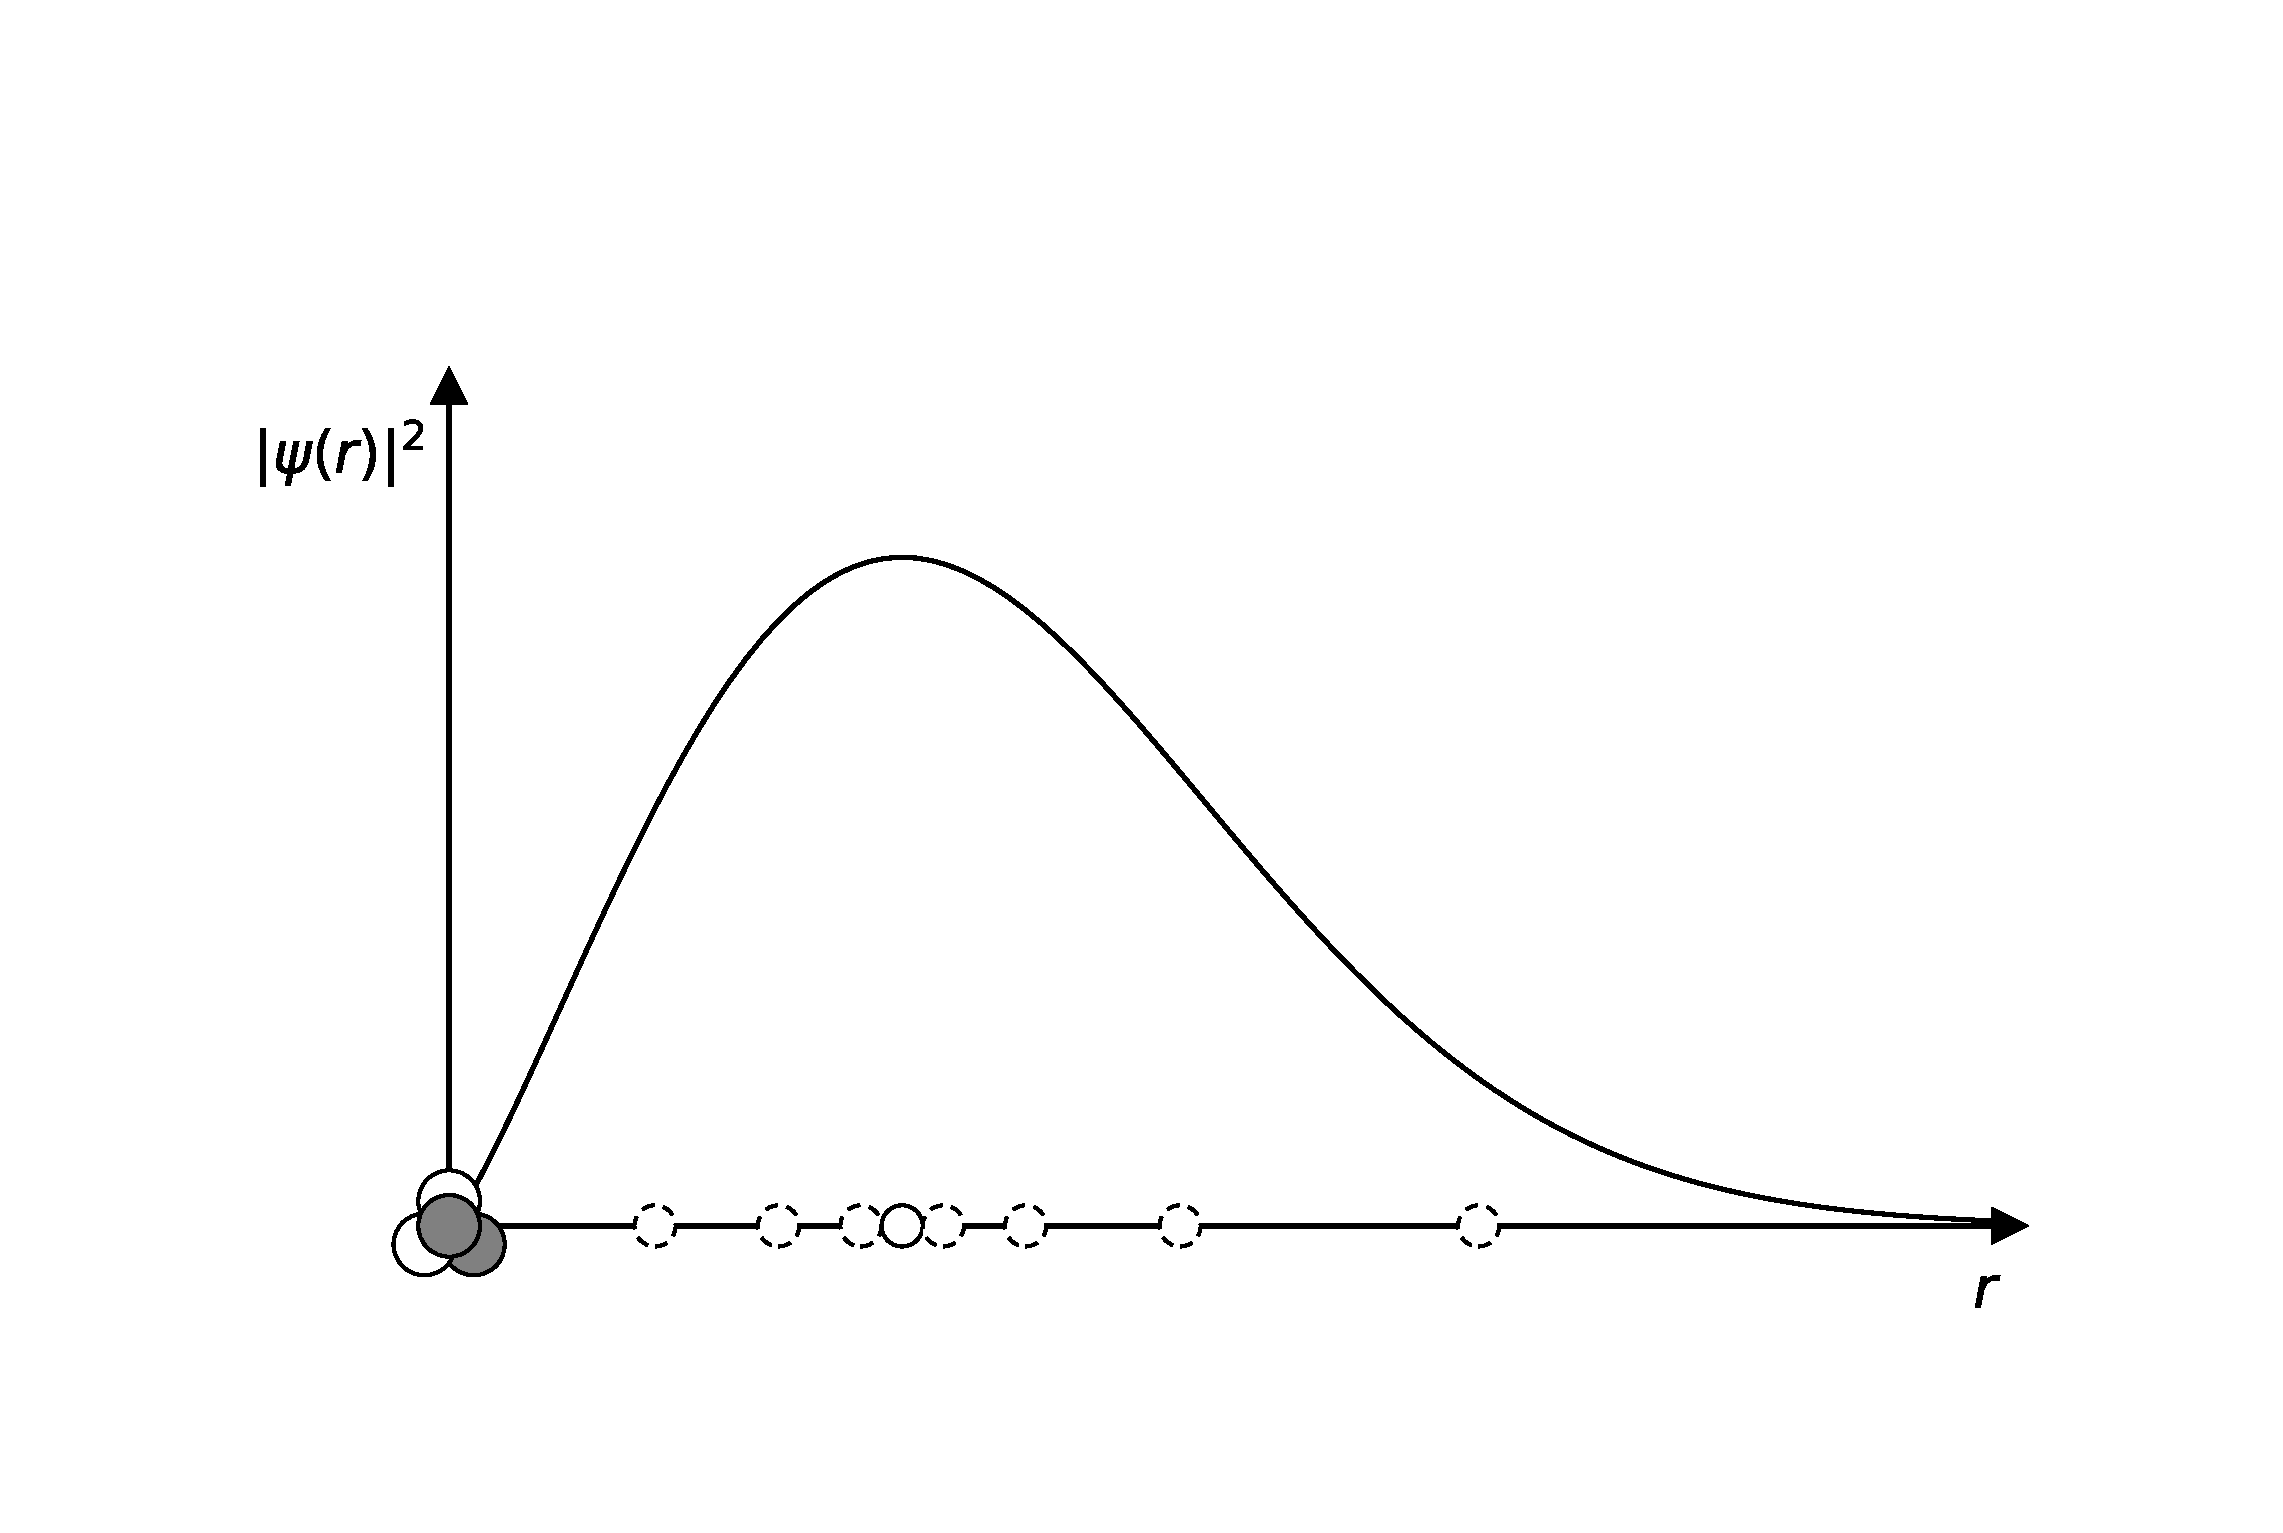
\includegraphics[scale=0.4]{images/radial_prob}
   \caption{Сферически симметричная плотность вероятности местонахождения электрона атома гелия как функция расстояния $r$ до ядра. Электрон может находиться не только в наиболее вероятном месте - точке максимума плотности, но и вообще в любом месте, хотя и с меньшей вероятностью.}
   \label{fig:radial_prob}
\end{figure}

Сделаем еще несколько замечаний относительно визуализации орбитали электрона, которая может быть довольно сложным трехмерным объектом.
Ее график как функции плотности распределения вероятностей находится в четырехмерном пространстве (три пространственные координаты и еще одна ось для ее значений), и представить его себе довольно проблематично.
Но если орбиталь, например, сферически симметрична, то о ней вполне можно судить по ее радиальной составляющей, то есть по ее зависимости от $r$ - расстояния до центра атома.
Так, например, для рассмотренного выше атома гелия радиальная составляющая плотности вероятности изображена на рис. (\ref{fig:radial_prob})).

\begin{figure}[t!]
   \centering
   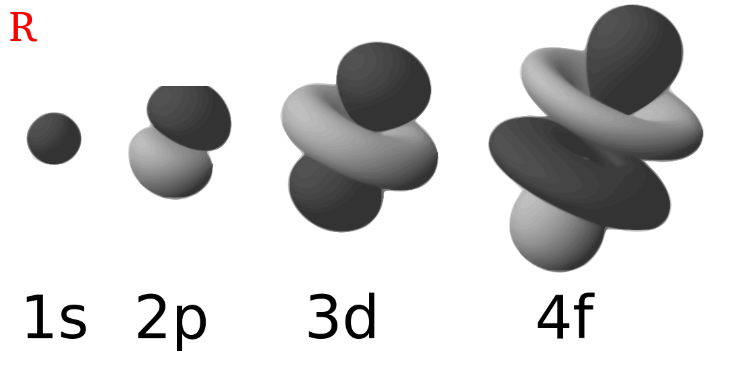
\includegraphics[scale=0.9]{images/electron_clouds_1}
   \caption{Различные виды электронных облаков.}
   \label{fig:electron_clouds_1}
\end{figure}

Иногда, желая придать положению электрона хоть какую-то конкретику, используют геометрическое представление орбитали - поверхность в пространстве, на которой плотность распределения вероятности имеет постоянное значение.
Значение выбирается либо максимальное, либо такое, что в ограничиваемой этой поверхностью области электрон может быть найден с вероятностью близкой к 1.

В случае атомов водорода и гелия эти фигуры представляют собой сферу с центром в ядре атома.
Это уже гораздо более наглядные геометрические образы, нежели абстрактные плотности распределения вероятностей.
Однако важно понимать, что они не определяют точные местоположения электрона в пространстве. 
В реальности электроны вовсе не двигаются по своим орбиталям по аналогии с движением планет Солнечной системы по своим орбитам.
Более того, само понятие движения электрона в данном случае весьма условно.
О конкретных координатах электрона, как и о траектории его движения по орбитали речи идти не может.

Наконец, электронное облако далеко не всегда имеет шарообразную форму.
Наиболее симметричная форма облака в виде простого шарового слоя как на рисунке \ref{fig:atom_1} может наблюдаться только у атомов водорода и гелия.
У других химических элементов формы электронных облаков гораздо сложнее и даже могут не иметь сферической симметрии.
На рис. (\ref{fig:electron_clouds_1}) изображено несколько примеров не сферически симметричных облаков.
Удивительно, но все эти замысловатые фигуры реализуются как некоторые решения уравнения Шреддингера.


\section*{Размеры}

Линейные размеры атома определить достаточно сложно из-за описанной выше неопределенности положения его электронов в пространстве.
О среднем радиусе атома принято судить либо по наиболее вероятной удаленности его электронов от ядра, либо по половине расстояния между ядрами двух одинаковых атомов в молекуле простого вещества.
В любом случае они неимоверно малы - от $31\cdot 10^{-12}$ метра (атом гелия) до $225\cdot 10^{-12}$ метра (атом цезия).
Порядком размера атома принято считать величину $1\mbox{\normalfont\AA} = 10^{-10}$ м (ангстрем).
Понять, насколько это мало, можно учтя, что атомов в капле воды примерно $4\cdot 10^{21}$, что вполне сравнимо с числом звезд во Вселенной.

Так как нуклоны в ядре упакованы довольно плотно, то о его размере вполне можно судить по размеру одного нуклона - около $0.86\cdot 10^{-15}$ метра (примерно одинаково для протонов и нейтронов). 
Таким образом, ядро в десятки - сотни тысяч раз меньше, чем весь атом.
Так, для простейшего атома водорода с радиусом порядка $53\cdot 10^{-12}$ метра и единственным протоном в ядре, электрон удален от центра на расстояние примерно в 100000 раз большее, чем само ядро \footnote{%
    Здесь, конечно же, имеется ввиду средняя удаленность электрона от ядра.
    О точном расстоянии до ядра говорить не приходится.}.
Таким образом, между протоном и электроном, где бы последний ни находился, расположено огромное количество пустоты.

Относительно размеров электрона даже в настоящее время известно очень немногое.
Последние попытки его определения показали, что оно не превосходит $10^{-20}$ метра.
В настоящее время электрон принято считать \textit{фундаментальной элементарной частицей}, то есть такой, которую пока не удалось разложить на составные частицы и определить ее размер.

В связи с этими числами обычно приводят следующий пример: если ядро атома увеличить до размеров теннисного мячика, то весь атом увеличится до размеров футбольного стадиона.
Электрон при этом станет не более чем песчинкой, спрятанной где-то в последних рядах стадиона без малейшего шанса его найти.

Наконец, учитывая тот факт, что орбитали электронов в атоме размазаны в пространстве, точно отделить атом от окружающей его пустоты практически невозможно.
При этом электронному облаку можно не приписывать сколько-нибудь существенного объема в силу того, что размер самих электронов по меньшей мере пренебрежимо мал, а наиболее вероятные места их пребывания сконцентрированы в тонких слоях.
Атомные ядра также имеют неимоверно малые размеры как сами по себе, так и по сравнению с размерами атомов.
Нуклоны, составляющие ядра, сами не плотны, а в свою очередь состоят из более мелких \textit{фундаментальных элементарных частиц}.

Таким образом можно сказать, что мы живем в практически пустом пространстве.
Все объекты, которые мы видим как абсолютно сплошные и непрозрачные, на самом деле на микроуровне весьма далеки от таковых.
Частицы их атомов расположены на весьма внушительных расстояниях друг от друга.
И все же этого оказывается достаточным, чтобы поглощать и испускать фотоны света, которые затем фиксируются нашими глазами и создают иллюзию сплошности объекта. 
Именно поэтому большинство объектов, которые мы видим, выглядят не размытыми и прозразрачными, а сплошными.


\section*{Масса, заряд и энергия}

Понятие орбитали тесно связано с понятием энергии.
Дело в том, что 

\begin{figure}[t!]
   \centering
   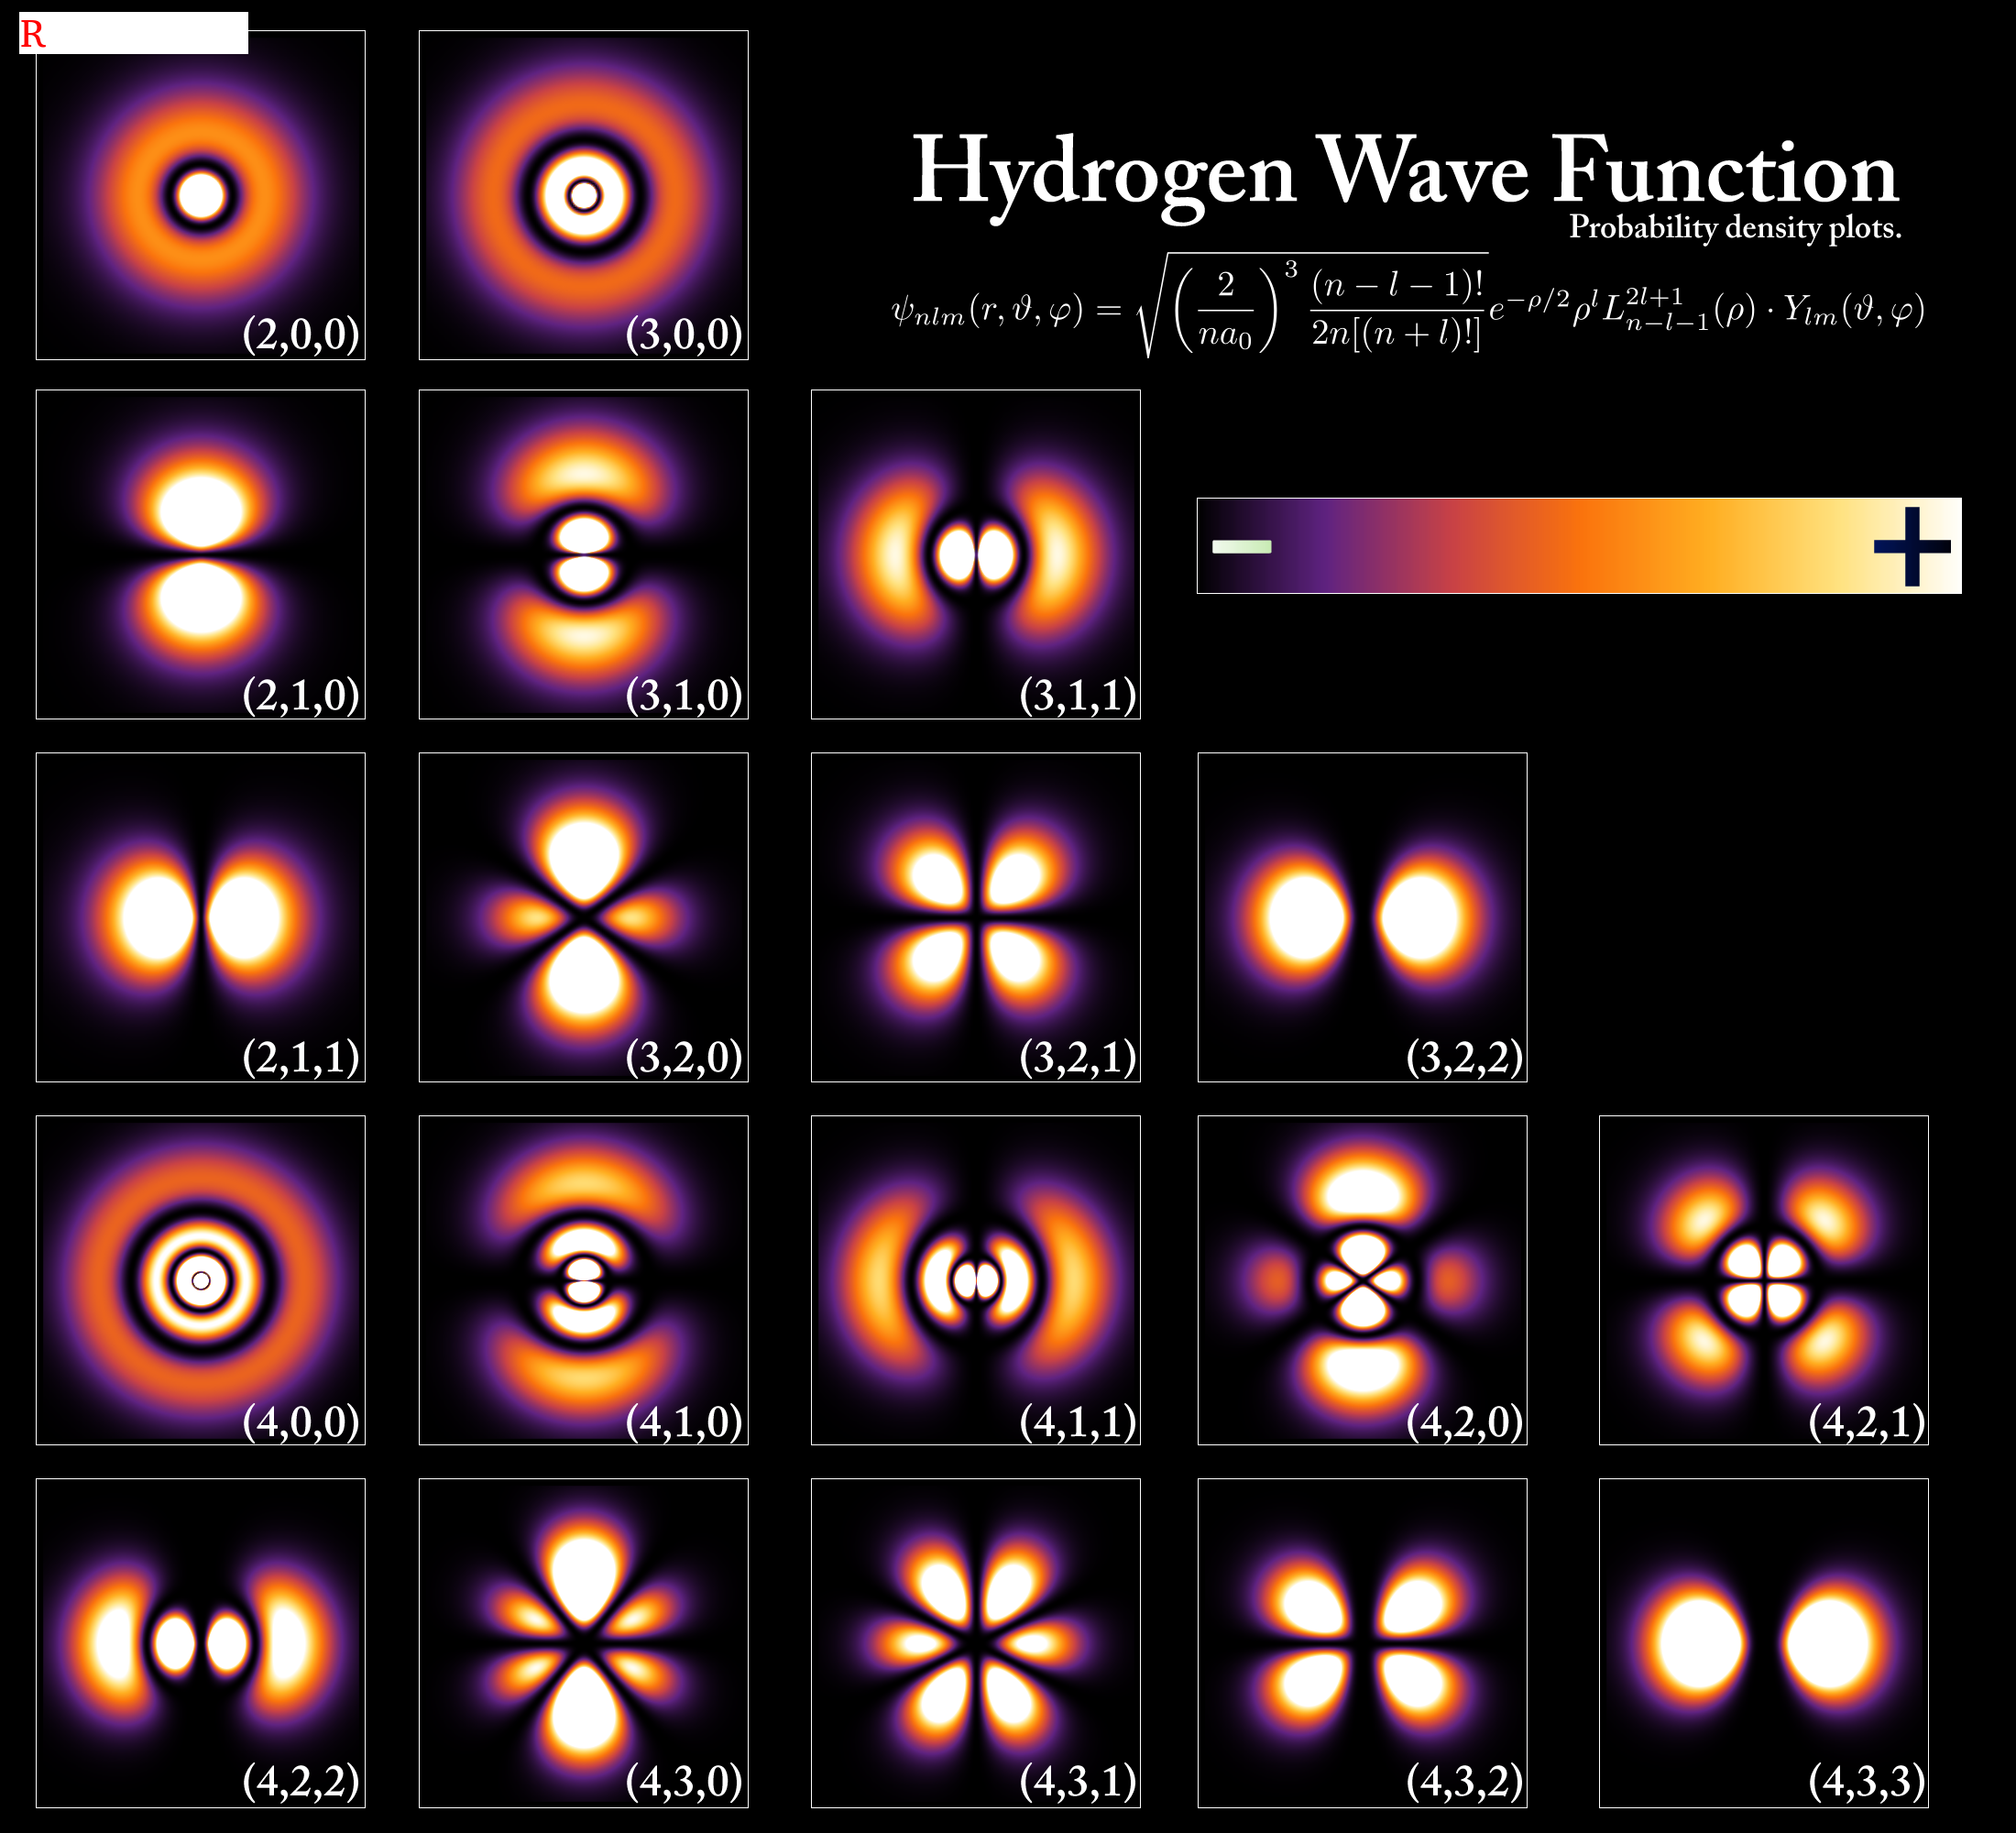
\includegraphics[scale=0.2]{images/hydrogen_electron_energy}
   \caption{Орбитали электрона атома водорода для различных значений энергии.}
   \label{fig:hydrogen_electron_energy}
\end{figure}



\section*{Уран}

Наиболее важными для нас являются примеры атомов урана и плутония, так как именно они выступают основными взрывчатыми веществами в атомном оружии.
Просуммируем все сказанное выше для атома урана.

Из 26 известных его изотопов только три встречаются в природе: \ce{^{234}_{92}U}, \ce{^{235}_{92}U}, \ce{^{238}_{92}U}.
Первый из них в силу своих слабых свойств почти не применяется.
Именно два последних имеют исключительное значение для производства ядерного оружия.
Более тяжелый \ce{^{238}_{92}U} наиболее распространен в природе ($99.27\%$).
Его сложнее расщепить и поэтому он не может напрямую использоваться как топливо в реакторах или рабочий материал атомной бомбы.
Вместо этого его используют в качестве отражателей нейтронов, существенно повышая общее выделение энергии при взрыве.

Наиболее ценный \ce{^{235}_{92}U} легче искусственно расщепить.
Именно благодаря этому именно он используется в качестве взрывчатого вещества в атомной бомбе.
Естественным образом в природе он встречается лишь в $0,72\%$ случаев, тогда как содержание его в бобме должно составлять не менее $80\%$.
Для его получения прибегают к процессу обогащения ... 

\begin{figure}[t!]
   \centering
   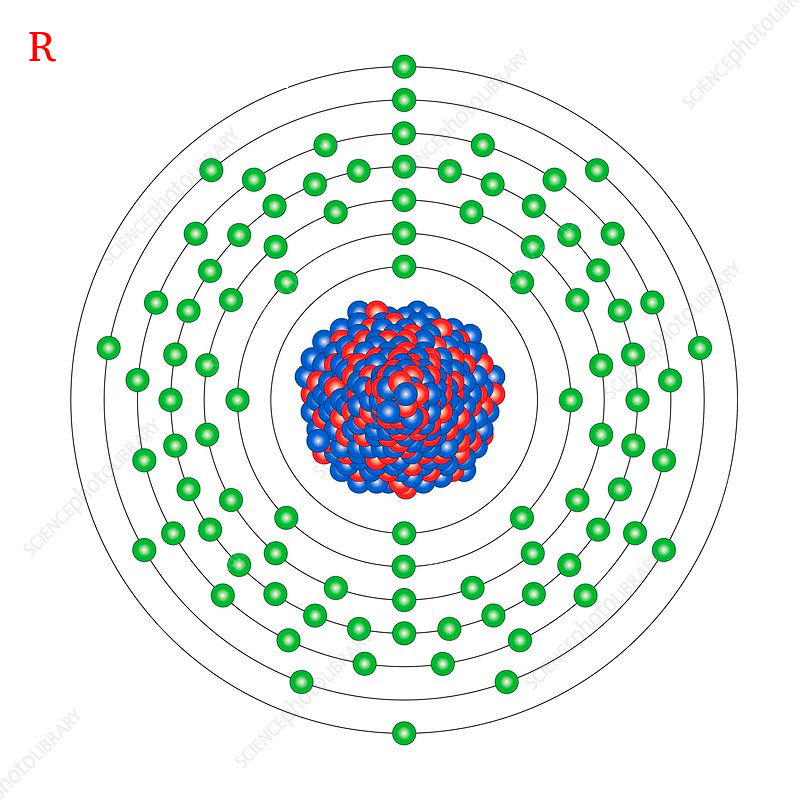
\includegraphics[scale=0.6]{images/uranium_1}
   \caption{Схематическое изображения атома урана-235.}
   \label{fig:uranium_1}
\end{figure}

На рисунке \ref{fig:uranium_1} схематически изображено строение атома \ce{^{235}_{92}U}, имеющего в своем ядре 92 протона и 143 нейтрона.
Все 92 электрона распределены между семью энергетическими уровнями (пунктирные линии на рисунке).
Каждый энергетический уровень включает в себя одну или более орбиталей, на каждой из которых находится один или два электрона.
Как было подробно описано выше, орбиталь - довольно сложный трехмерный объект, отражающий вероятность электрона находиться в том или ином месте пространства. 
Всего электронная оболочка атома урана имеет 48 орбиталей, лишь первая из которых (самая близкая к ядру) имеет простую шарообразную форму, как на рисунке \ref{fig:atom_1}.
Остальные имеют более сложную форму.

Приблизительный радиус атома урана - $175\cdot 10^{-12}$ метра, что примерно в 3 раза больше атома водорода.


Изобразить точно орбитали электронов атома урана крайне затруднительно ввиду того, что каждый электрон взаиможействует со всеми остальными, несколько искажая картину их орбиталей.
Если для одного-единственного электрона в атоме водорода картина более-менее простая, то в присутствии множества электронов представить совместное электронное облако практически невозможно.
  





[подробнее о числах для Урана (отдельная секция?)]
[картинка атома урана]
[валентные электроны - на внешней оболочке каждого энергетического уровня]


\section*{Стабильность и распад}

Итак, устройство атома в целом должно быть достаточно понятно.
Но почему же он стабилен?
Почему электроны, протоны и нейтроны образуют целостную структуру, не разлетаясь в разные стороны и не сталкиваясь друг с другом?


Почему, например, электроны не падают на ядро, а нейтроны не сталкиваются с протонами и не разлетаются в разные стороны?


Чтобы атом мог существовать сколько-нибудь продолжительное время, между его протонами, нейтронами и электронами должны действовать некоторые силы.
Именно эти силы и делают атом стабильной структурой.
Эти силы не дают частицам, с одной строны, разлететься в разные строны, а с другой - упасть друг на друга.



Как было сказано выше, атомы одного и того же химического элемента всегда имеют фиксированное число протонов, но могут иметь разное число нейтронов. 
Эти обеспечивается разнообразие ...
Главное, помимо массы, различие разных изотопов одного и того же элемента - их стабильность, о чем рассказано ниже.



В среднем число нейтронов для изотопов данного химического элемента не слишком отличается от числа протонов, которое для него определено однозначно.
Число нейтронов у изотопа может быть как меньше, так и больше числа протонов.
В обоих случаях, чем больше эта разница, тем неустойчивее атом становится и тем выше вероятность ему распасться на атомы более легких элементов.
Если число нейтронов отличается от 

Выше было рассказано о неустойчивости разных изотопов и естесственной радиоактивности...
Это явления имеет ключевое значени для искусстевенного расщепления ядра атома...


Стабильность атома определяется через \textit{период полураспада} - время, за которое распадутся ядра 




Простейшим из атомов является атом водорода, обладающий минимальным числом протонов - одним.
Число нейтронов в атоме водорода может быть от нуля до семи, но с ростом их числа ядро становится нестабильным и быстро спонтанно распадается.
Так, у трития - изотопа водорода с тремя протонами, период полураспада составляет около 12 лет, а у квадия с четырьмя протонами - всего $1.4\cdot 10^{−22}$ секунды.
Это же верно для любых атомов.
Нейтроны необходимы, чтобы стабилизировать пытающиеся разлететься протоны, но с ростом их числа атом все-таки теряет стабильность (см. рис. \ref{fig:atom_stability}).


\begin{figure}[t!]
   \centering
   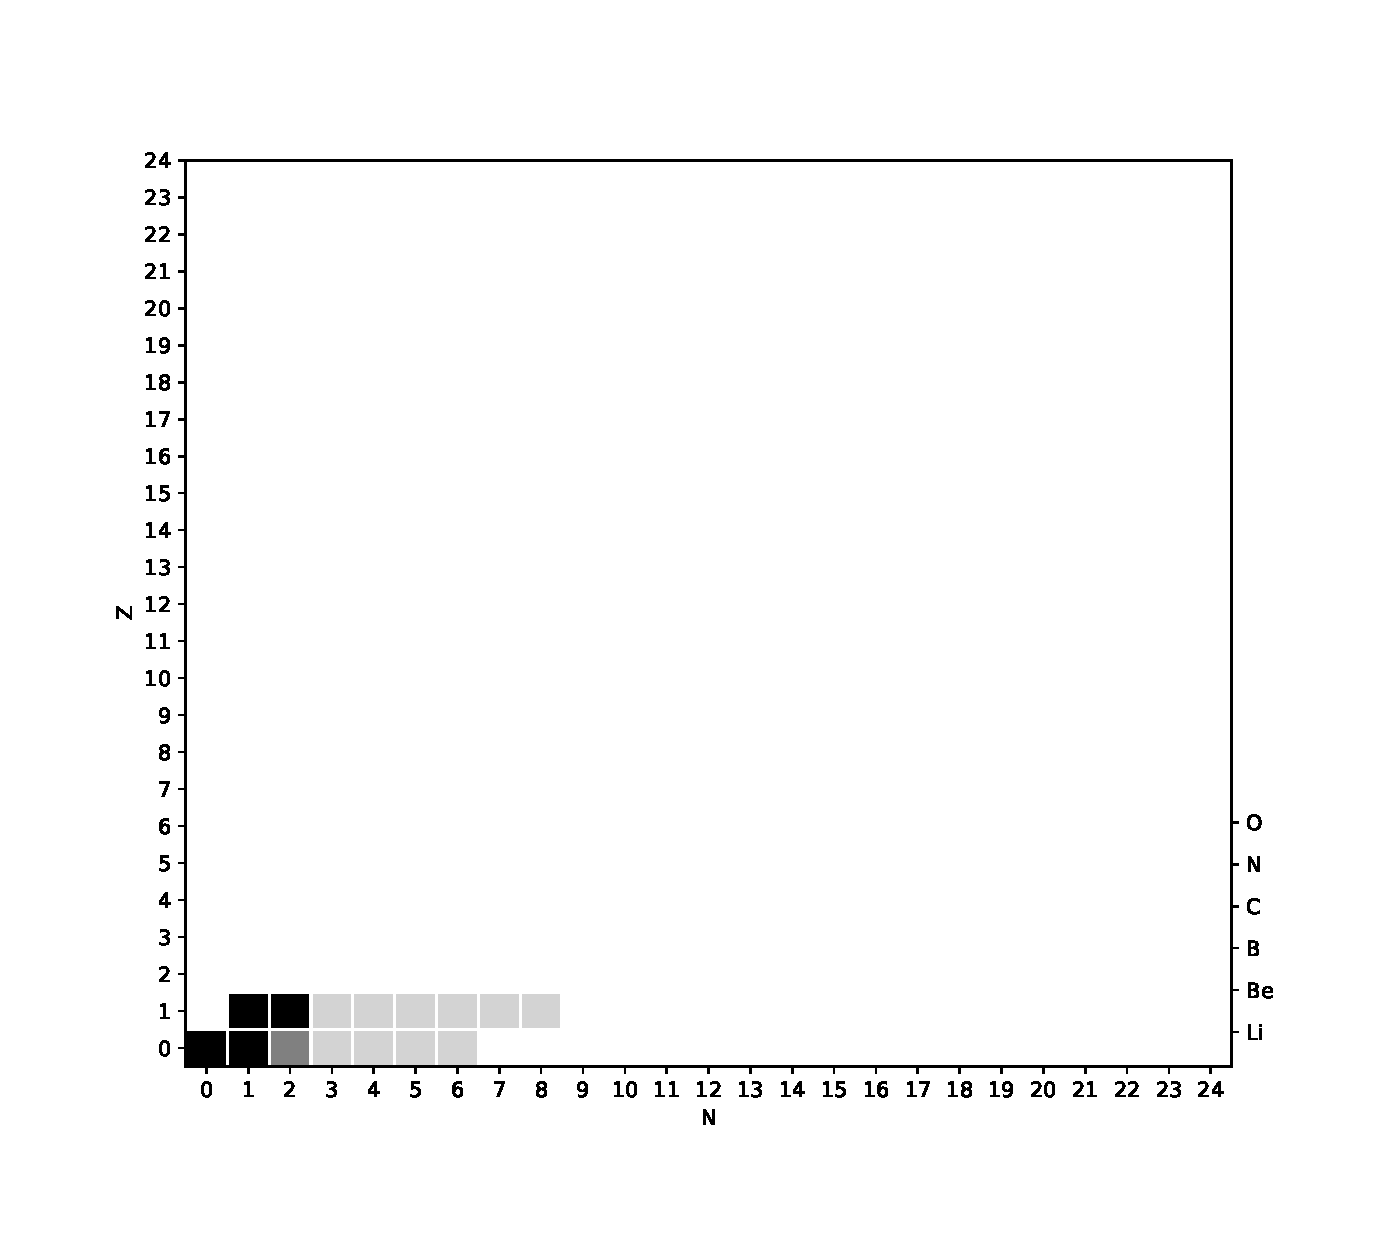
\includegraphics[scale=0.4]{images/atom_stability}
   \caption{Фрагмент диаграммы стабильности атомов химических элементов в зависимости от числа протонов и нейтронов в ядре. Темные клетки - стабильные атомы, светлые - относительно стабильные атомы, живущие от часов до миллиардов лет, пустые - нестабильные атомы, живущие не более малых долей секунд.}
   \label{fig:atom_stability}
\end{figure}




Электроны и протоны являются носителями электрического заряда, нейтроны электрически нейтральны. 
Электроны отрицательно заряжены, протоны - положительно, причем заряд электрона равен заряду протона, а числа электронов и протонов в атоме равны, так что атом оказывается электронейтральным в целом.
Бывает, что атом теряет или приобретает электроны, приобретая таким образом заряд и новое название - ион.
Здесь нас будут интересовать только атомы, не имеющие заряда.

При массе атома от $1.7\cdot 10^{-27}$ кг (атом Водорода-1) до $209.6\cdot 10^{-27}$ кг (атом свинца-208) масса одного электрона составляет всего $9.1\cdot 10^{-31}$ кг.
То есть в ядре сконцентрировано более $99.9\%$ всей массы атома.
Интересно, что кварки, из которых состоят протон, дают менее $2\%$ его массы, основная же часть массы протона приходится на виртуальные частицы.
Нам далее не потребуются столь глубокие субатомные понятия, как кварки и виртуальные частицы. 
Многие из них были открыты и изучены уже после Манхэттенского проекта и никак на него не повлияли. 


\section*{Цепные реакции}

Химические превращения одних веществ в другие происходят только путем перегруппировки атомов между их молекулами.
В процессе химической реакции молекулы исходных веществ отдают или принимают атомы, в результате образуя молекулы новых веществ. 
Сами атомы при этом остаются неизменными.
В этом смысле атом действительно является \textit{наименьшим} носителем химических свойств данного вещества, как и думали древние.

Таким образом, одних простых химических реакций недостаточно, чтобы решить главную задачу алхимии - заставить атомы одного вещества стать атомами другого.
Для того чтобы атомы одного вещества превратились в атомы другого, необходимо более грубое физическое вмешательство - ядерные реакции, в процессе которых ядра атомов взаимодействуют друг с другом или с элементарными частицами.
В результате ядерных реакций тяжелые атомы могут распадаться в более легкие (реакции деления), либо соединяться в еще более тяжелые (реакции синтеза).
Оба этих типа реакций происходят с выделением огромного количества тепла и радиации, что и послужило главной причиной для использования их в военных целях.

------------------------

сколько энергии выделяется при распаде одного этома...





------------------------ IDEAS ------------------------ 



Мы не будет углубляться 
Для общего понимания устройства и принципа работы ядерного оружия знать как устроены протоны и нейтроны необязательно. 
Не было о них известно и во времена Манхэттенского проекта.


